\documentclass[11pt,a4paper]{article}
\usepackage[utf8]{inputenc}
\usepackage[T1]{fontenc}
\usepackage[spanish,es-nodecimaldot]{babel}
\usepackage{lmodern,amsmath,amssymb,graphicx,booktabs,float,xcolor,caption}
\usepackage[margin=2.2cm]{geometry}
\usepackage{url}
\makeatletter\g@addto@macro{\UrlBreaks}{\do\-\do\_\do\.}\makeatother
\urlstyle{tt}\DeclareRobustCommand{\archivo}[1]{\path{#1}}
\usepackage[colorlinks=true,linkcolor=blue!50!black,urlcolor=blue!50!black]{hyperref}
\captionsetup{font=small,labelfont=bf}
\graphicspath{{../figuras/}}
\newcommand{\aviso}[1]{\par\smallskip\noindent\fcolorbox{orange!70!black}{orange!8}{\parbox{\dimexpr\linewidth-2\fboxsep-2\fboxrule}{\small #1}}\par\smallskip}
\newcommand{\tabla}[1]{\input{tablas/#1}}

\title{Simulación MEIGA del montaje con la fuente $^{241}$Am-Be\\
\large entrada lateral (haz, halo y fondo), calibración con muones y comparación con el prototipo}
\author{Jaime Betancourt}
\date{22 de octubre de 2026}

\begin{document}
\maketitle

\begin{abstract}
Se simuló en MEIGA el montaje real del prototipo con la fuente de $^{241}$Am-Be: un millón de neutrones que
entran \emph{por el costado} del tanque, repartidos según el modelo del blindaje (haz directo 35\,\%, halo
difuso 45\,\%, fondo hemisférico 20\,\%), en agua pura y en agua con 2.5 y 10\,\% NaCl, con el PMT de
Sidelnik y sin S($\alpha,\beta$). Por neutrón incidente, la eficiencia de señal ($Q\geq1$~p.e.) es 17.5\,\% en
agua pura, 22.7\,\% con 2.5\,\% NaCl y 29.8\,\% con 10\,\% NaCl, y la carga media de la señal pasa de 1.95 a
3.93 y 5.30~p.e. Con una corrida de 2000
muones verticales de 4~GeV/c en el mismo detector se calibró el prototipo con el pico de muones de las tomas
de fondo: \textbf{7.9~p.e. por cada 1000~ADC} (7.5--8.6 entre tomas y métodos), el doble de los 3.95 usados
hasta ahora. Con esta calibración el disparo del prototipo ($\approx$3000~ADC) equivale a $\approx$24~p.e.
La simulación predice que casi ningún neutrón da tanta luz, mientras que el exceso medido con la fuente está
entre 0.08 y 0.7~VEM y es $10^3$--$10^4$ veces mayor que lo predicho para 1~Ci. Las tomas son
internamente coherentes: la región de muones se resta a cero en los tres medios. La discrepancia, por tanto,
no se resuelve con la calibración y apunta a un efecto que la simulación no contiene. Con 10\,\% NaCl el
cuadro es el mismo: el exceso medido es unas 4\,000--5\,000 veces lo predicho, y la forma de su espectro casi no
cambia con la sal, mientras que en la simulación se alarga un factor 4. Con el método de los cuadernos del prototipo
(un factor horizontal y uno vertical libres pero comunes a los tres medios) el montaje reproduce el agua pura y
los medios con sal dentro de un factor 2, con $\approx$1000~ADC/p.e.\ y $5$--$7\times10^6$ neutrones en 300~s; ese
factor es unas 8 veces el que dan los muones.
\end{abstract}
\tableofcontents

\section{Corridas}
Todas se hicieron en el contenedor \texttt{silly\_roentgen} del portátil, con Geant4 + MEIGA, física
\texttt{QGSP\_BERT\_HP\_\allowbreak NoThermal} (sin S($\alpha,\beta$)), detector SaltyWCD (agua $R=48$~cm,
$H=133$~cm, Tyvek 0.12~mm con reflectividad escalada por 0.94, acero 0.5~mm) y el PMT de Sidelnik
(elipsoide de Pyrex de $10.16\times10.16\times5$~cm en la tapa). La inyección es \texttt{eFromFile}; como
\archivo{ParticleFiller.cc} guarda $(p_x,p_y,-p_z)$, los archivos se escriben con $p_z$ invertido.

\begin{table}[H]\centering\footnotesize\setlength\tabcolsep{4pt}
\begin{tabular}{lllrrr}
\toprule
Corrida & Material, $\rho$ [g/cm$^3$] & Partículas & Tiempo & Disco & Archivos \\
\midrule
Montaje, agua pura & \texttt{Water\_TS\_H\_of\_Water}, 0.99820 & $10^6$ n & 10\,463 s & 62.3 GB & 98 \\
Montaje, 2.5\,\% NaCl & \texttt{SaltyWater\_NaCl\_2.5pct}, 1.01604 & $10^6$ n & 12\,918 s & 102.1 GB & 98 \\
Montaje, 10\,\% NaCl & \texttt{SaltyWater\_NaCl\_10.0pct}, 1.07051 & $10^6$ n & $\approx$16\,900 s & 149.6 GB & 99 \\
Muones VEM & agua pura & 2000 $\mu^-$, 4 GeV/c & 5\,827 s & 53.7 GB & 70 \\
\bottomrule
\end{tabular}
\caption{Corridas. Cada corrida de neutrones se partió en 4 partes de $\approx$250\,000 eventos. Los resultados
están en el disco ADATA (\archivo{Corrida-*-resultados}), verificados con número de archivos, bytes y md5
del listado. El tiempo de 10\,\% se estimó con las fechas de los archivos de salida.}
\end{table}

\paragraph{Neutrones de entrada.} El mismo archivo (\archivo{1000000N-AmBe-montaje-haz-halo-fondo.txt})
se usó en todos los medios, para que la comparación sea evento a evento:
haz directo (350\,000 n) con el espectro ISO~8529 (0.1--10.8~MeV), desde la posición de la fuente
$(-88.06, 0, 66.56)$~cm en un cono de 2.86°; halo difuso (450\,000 n) de 0.5~eV a 100~keV con espectro
$1/E$, desde la cara del plomo ($120\times40$~cm) con ley del coseno; fondo hemisférico (200\,000 n),
maxwelliano de $kT=25.3$~meV entre $10^{-4}$ y 0.5~eV, desde un plano de $96\times133$~cm frente al tanque.
Para escalar a la fuente real se usa el modelo de 5~minutos de 1~Ci: 130\,711 (haz), 167\,963 (halo) y
74\,598 (fondo) neutrones que llegan al tanque.

\paragraph{Verificación.} Antes de cada corrida completa, una prueba de 30 neutrones comprobó, en el registro
de MEIGA, el material, la fracción de NaCl, la densidad, la física sin térmica, el tamaño del tanque y que
posición y momento inyectados coinciden con el archivo. Al procesar (\archivo{scripts/procesar_montaje.py})
se comprueba que cada parte tiene tantas cargas como líneas de entrada y que la energía del primer paso de
cada neutrón coincide con la del archivo (diferencia relativa máxima $6\times10^{-4}$).
En los muones las cuatro partes suman 2000 eventos (501/500/500/499, por el reparto de \texttt{split}) y todos
dejan carga.

\section{Respuesta del detector a la entrada lateral}
La tabla~\ref{tab:comp} da, por componente, la eficiencia de señal, la fracción de neutrones capturados en el
medio activo ($\eta_\text{cap}$), la carga media de los eventos con señal y la mediana del tiempo de captura.
La columna ``pred.\ tapa'' es la predicción del informe anterior (corridas con inyección vertical por la tapa
y Campaña~1).

\begin{table}[H]\centering\small
\tabla{respuesta_componentes}
\caption{Respuesta por componente con entrada lateral. $\varepsilon$: fracción de neutrones incidentes con
carga $\geq1$ o $\geq12$~p.e.; $\eta_\text{cap}$: fracción con al menos una captura en el agua; $\langle
Q\rangle$: carga media de los eventos con $Q\geq1$.}\label{tab:comp}
\end{table}

\begin{itemize}
\item La entrada lateral da \textbf{menos señal que la entrada por la tapa}: 29.8 frente a 36.4\,\% para
el haz en agua pura y 11.4 frente a 17.7\,\% para el halo. La carga media es la mitad (1.9 frente a 3.5~p.e.):
las capturas ocurren cerca de la pared lateral, lejos del PMT de la tapa.
\item Con 2.5\,\% NaCl la eficiencia total sube de 17.5 a 22.7\,\% y la carga media se duplica (1.95 a
3.93~p.e.), por las cascadas del $^{36}$Cl (35.4\,\% de las capturas). La fracción con $Q\geq12$~p.e.\ pasa de
0.05 a 1.35\,\%: un factor 25.
\item Con 10\,\% NaCl la eficiencia total llega a 29.8\,\% y la carga media a 5.30~p.e.; el $^{35}$Cl
recibe el 67.5\,\% de las capturas y la fracción con $Q\geq12$~p.e.\ sube a 2.99\,\% (56 veces la de agua
pura). La fracción de neutrones capturados en el agua pasa de 40.2 (pura) a 43.3 (2.5\,\%) y 49.0\,\% (10\,\%).
\item La mediana del tiempo de captura baja de 104 (pura) a 79 (2.5\,\%) y 47~$\mu$s (10\,\%).
\end{itemize}

\begin{table}[H]\centering\small
\tabla{nucleos_modelo5min}
\caption{Núcleo de la primera captura en el medio y número esperado de eventos para la fuente de 1~Ci en
5~min (modelo del blindaje), con la respuesta lateral simulada.}
\end{table}

\begin{figure}[H]\centering
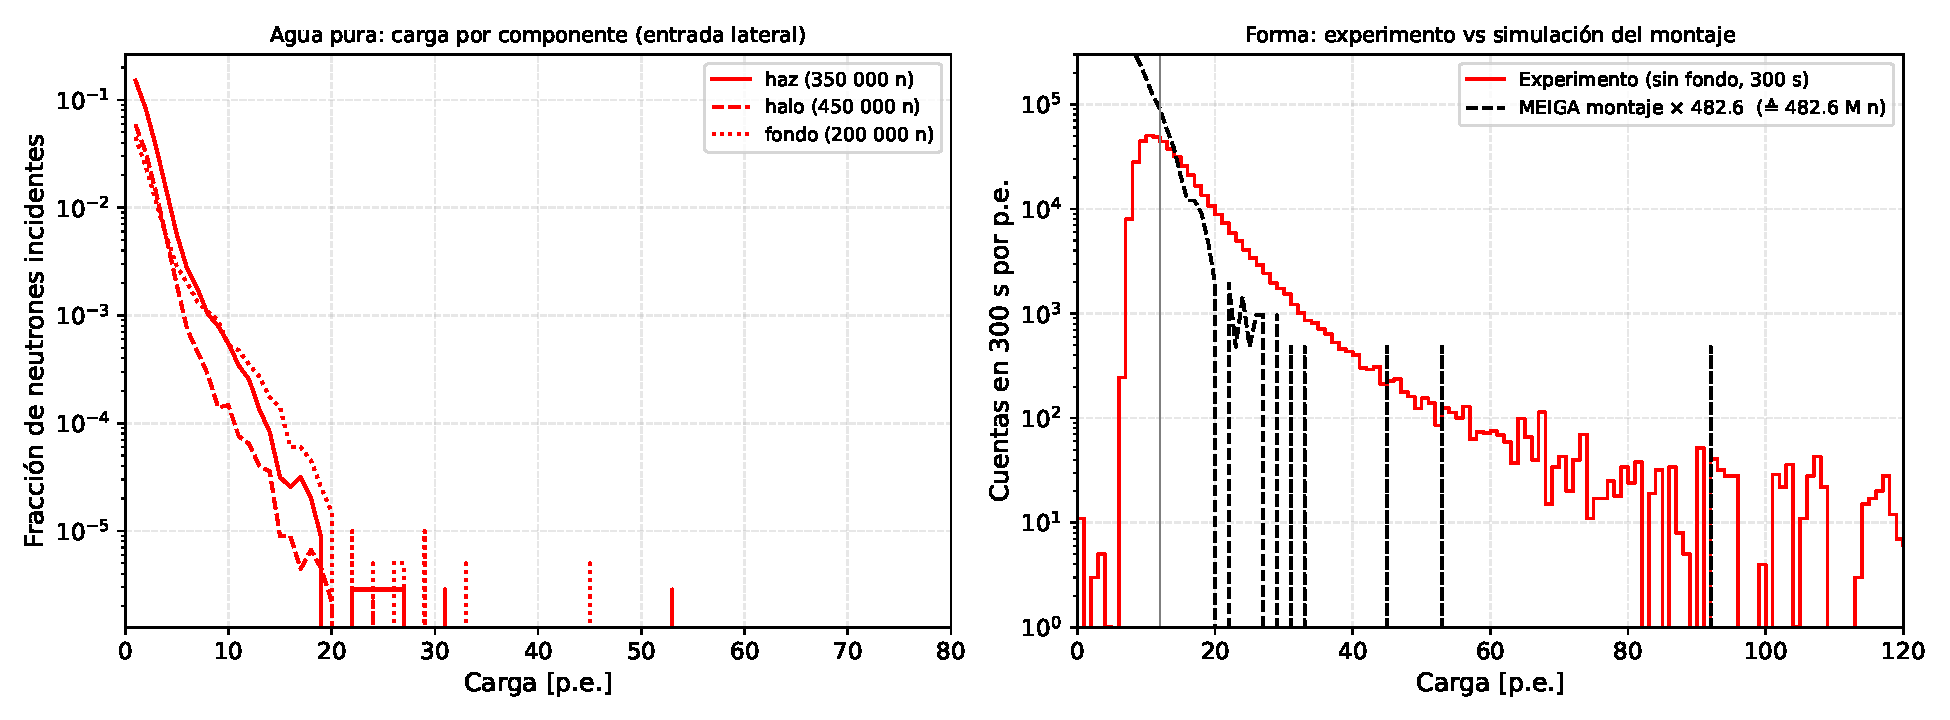
\includegraphics[width=\linewidth]{fig01_carga_pura.pdf}
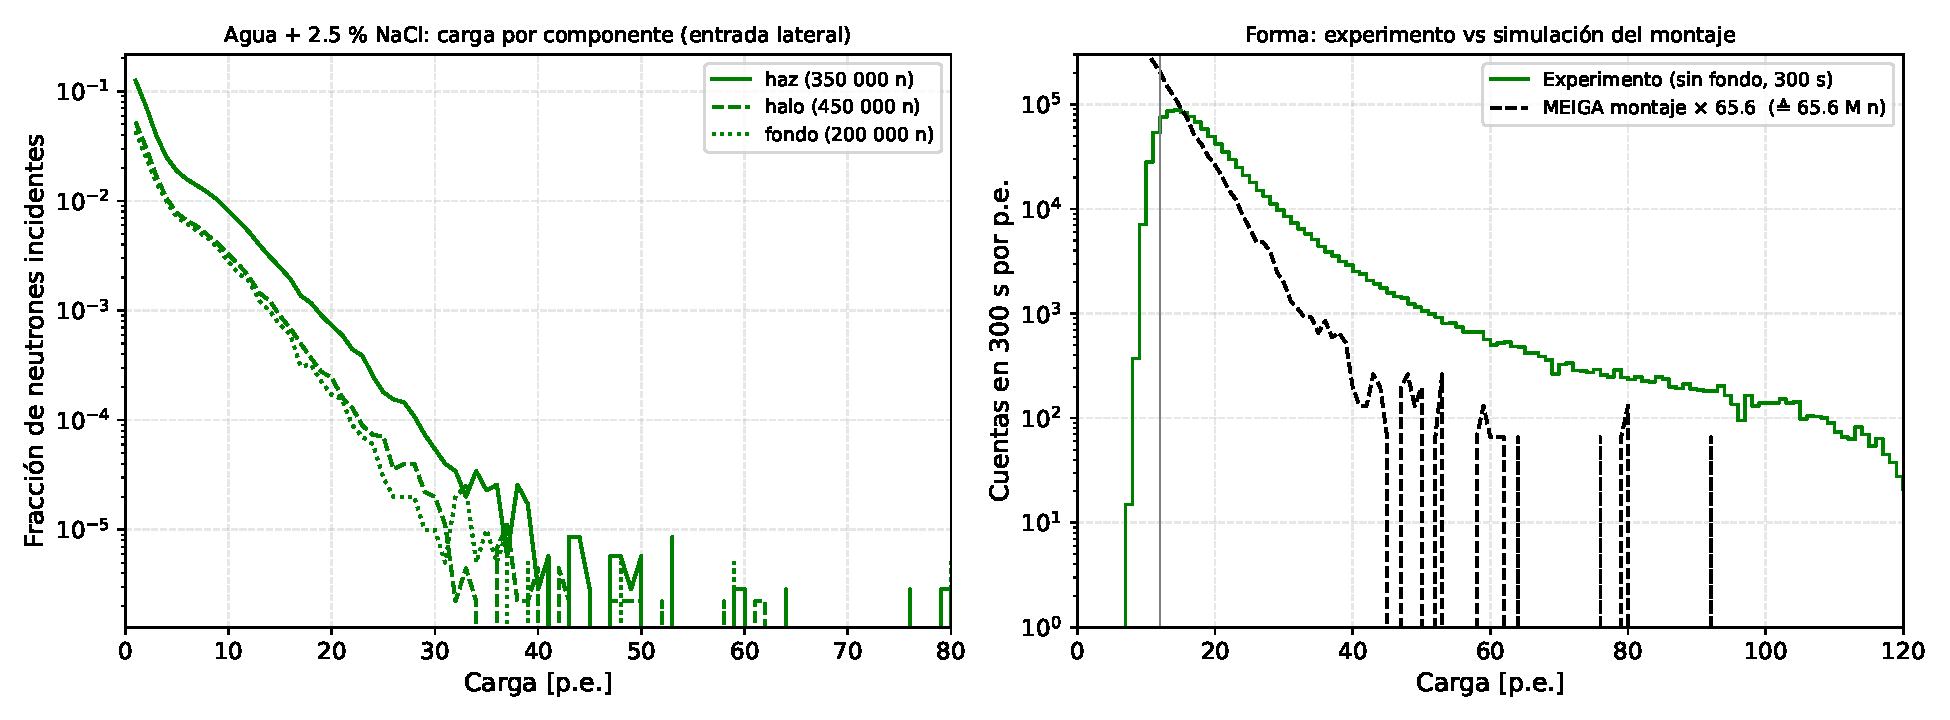
\includegraphics[width=\linewidth]{fig01_carga_nacl25.pdf}
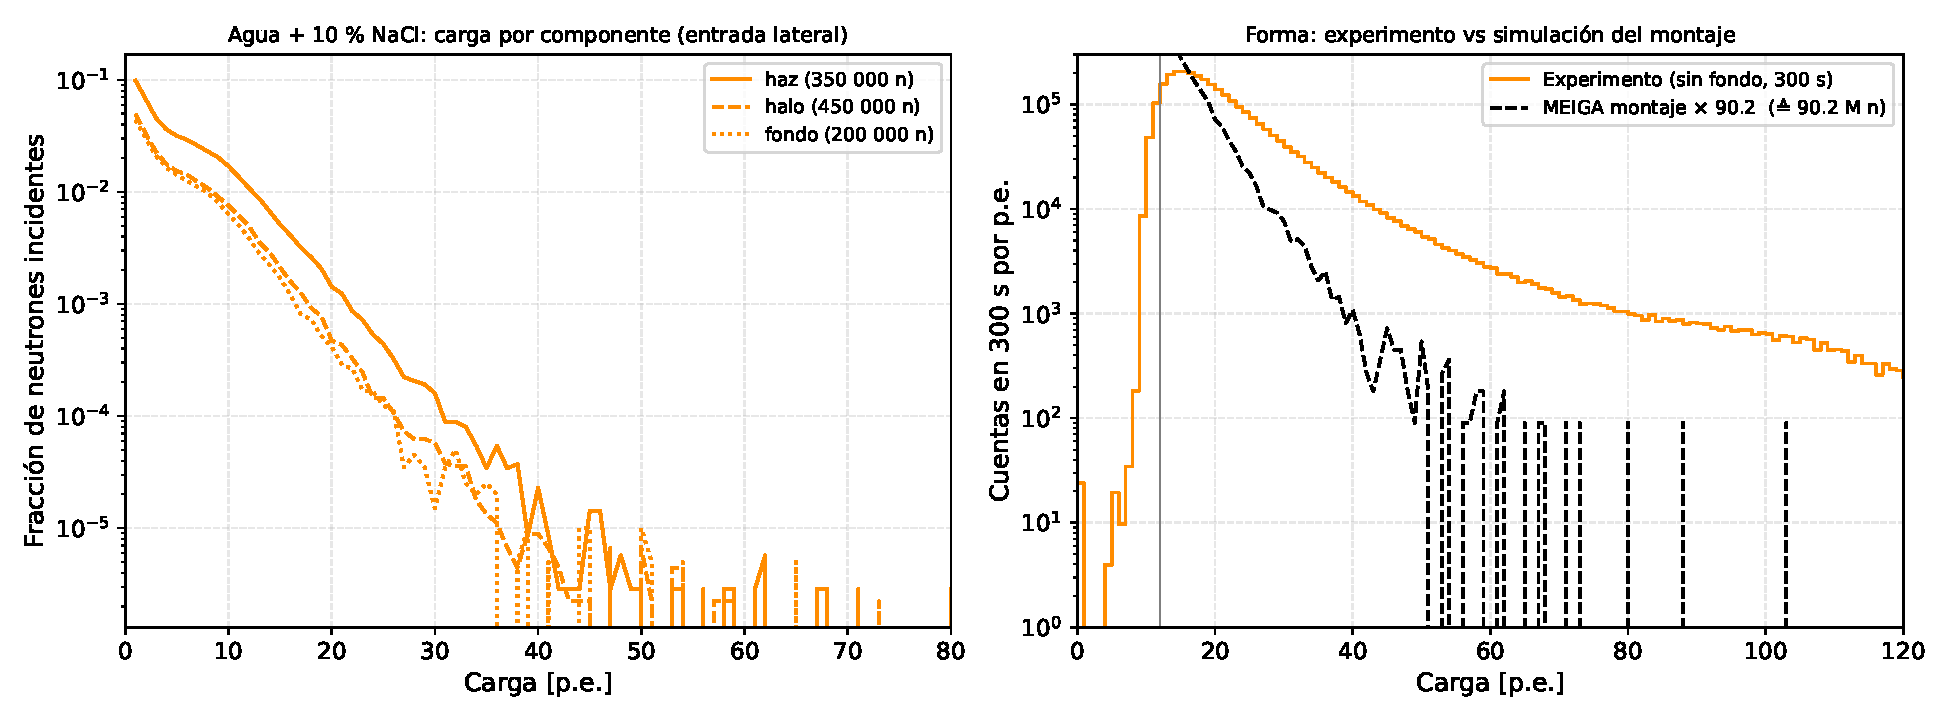
\includegraphics[width=\linewidth]{fig01_carga_nacl10.pdf}
\caption{Izquierda: distribución de carga por componente (por neutrón incidente). Derecha: forma del exceso
medido (con la calibración antigua, 3.95~p.e./kADC) y de la simulación escalada para coincidir entre 12 y
60~p.e. Agua pura (arriba), 2.5\,\% NaCl (centro) y 10\,\% NaCl (abajo). La simulación cae a cero hacia
20--50~p.e.; el experimento sigue más allá de 100~p.e.}\label{fig:carga}
\end{figure}

\section{Calibración p.e./ADC con muones}
El prototipo se calibraba con 3.95~p.e.\ por cada 1000~ADC (cuaderno del detector). Para comprobarlo se
simularon 2000 $\mu^-$ verticales de 4~GeV/c que entran por la tapa en un disco de radio 45~cm y atraviesan
los 133~cm de agua, en el mismo detector y con el mismo PMT. La carga simulada por muón tiene el pico en
\textbf{305~p.e.} (media 325, mediana 313; 68\,\% entre 284 y 362~p.e.). El pico de muones de cada toma de
fondo se encontró con el mismo algoritmo (histograma suavizado y parábola en el máximo), con los dos métodos de
carga del prototipo (ventana del disparo y carga positiva de toda la traza, ``robusto'').

\begin{table}[H]\centering\small
\tabla{calibracion_vem}
\caption{Calibración por el pico de muones (VEM simulado = 305~p.e.).}\label{tab:cal}
\end{table}

\begin{figure}[H]\centering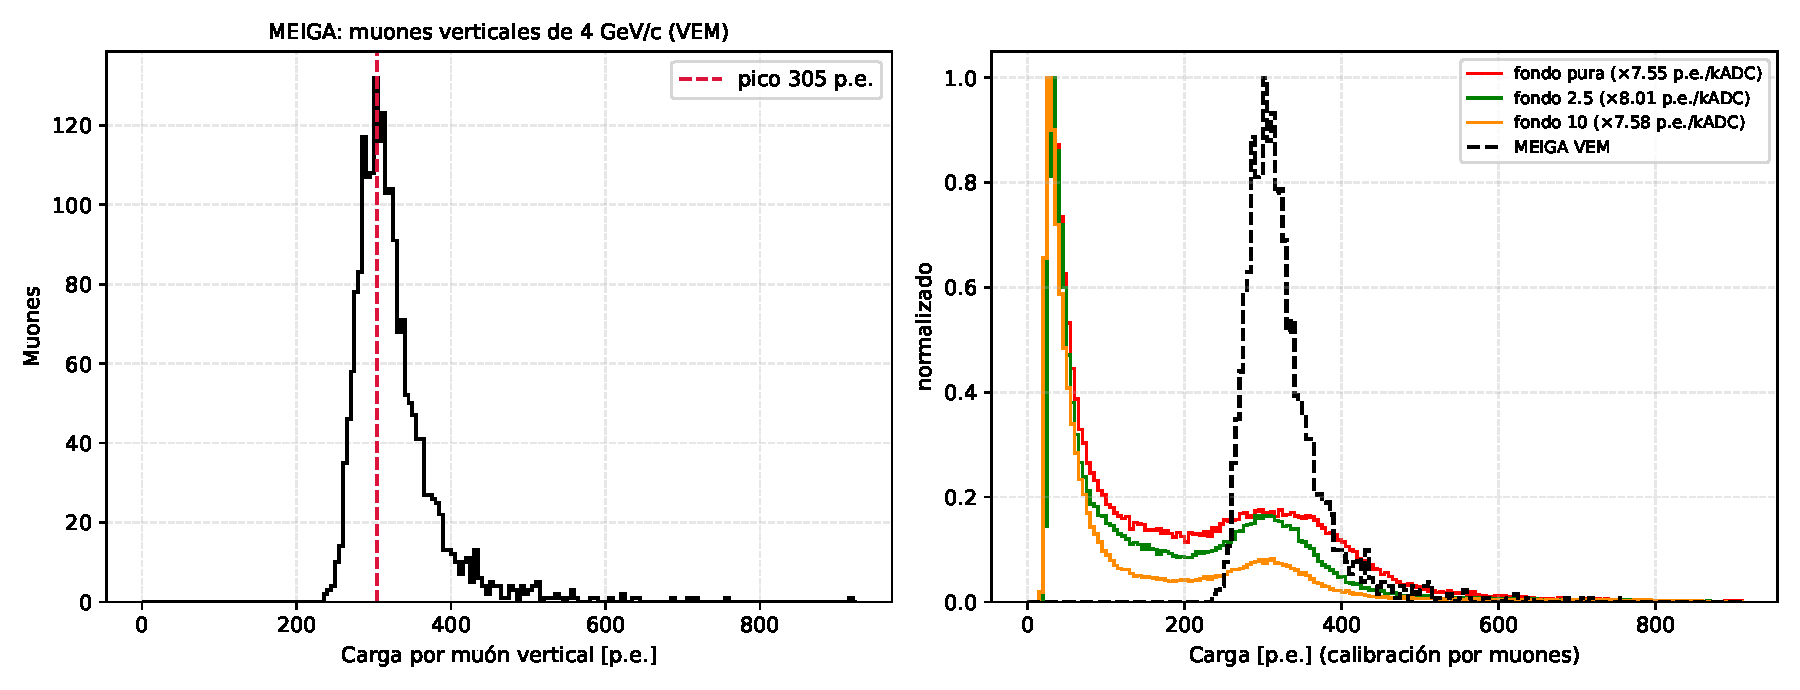
\includegraphics[width=\linewidth]{fig05_calibracion_vem.pdf}
\caption{Izquierda: carga de los 2000 muones verticales simulados. Derecha: tomas de fondo convertidas a
p.e.\ con su calibración, comparadas con los muones simulados.}\label{fig:vem}
\end{figure}

Las seis determinaciones coinciden entre sí dentro del 7\,\%: \textbf{7.9~p.e./kADC, unos 127~ADC por
p.e.} El pico medido es más ancho que el simulado porque el fondo contiene muones de todas las direcciones
(trazas más largas y más cortas) y otras partículas de la cascada; esa diferencia de longitud de traza da
una incertidumbre del orden del 10\,\% en la calibración. Con la calibración por muones:
\begin{itemize}
\item el disparo del prototipo, $\approx$3000~ADC (percentil 1 de las cargas medidas), equivale a
\textbf{$\approx$24~p.e.}, no a 12;
\item 1~VEM $\approx$ la luz de una traza vertical de 133~cm, unos 270~MeV de electrón equivalente:
$\approx$1.1~p.e.\ por MeV, coherente con los $\approx$2~p.e.\ que dan en la simulación los gammas de
2.2~MeV de la captura en H.
\end{itemize}

\section{Experimento frente a simulación con la nueva calibración}
\subsection{Coherencia de las tomas}
La figura~\ref{fig:bandas} y la tabla~\ref{tab:bandas} comparan, en p.e.\ y en VEM, las tasas de la toma con
fuente y de la toma de fondo de cada medio. \textbf{Por encima de $\approx$0.9~VEM (280~p.e.) las dos tomas
coinciden en los tres medios} (cocientes de 1.01 a 1.2): la ganancia, la duración y la normalización de las
tomas son coherentes, y la resta del fondo es correcta. El exceso de la fuente está entre el disparo y
$\approx$0.7~VEM.

\begin{figure}[H]\centering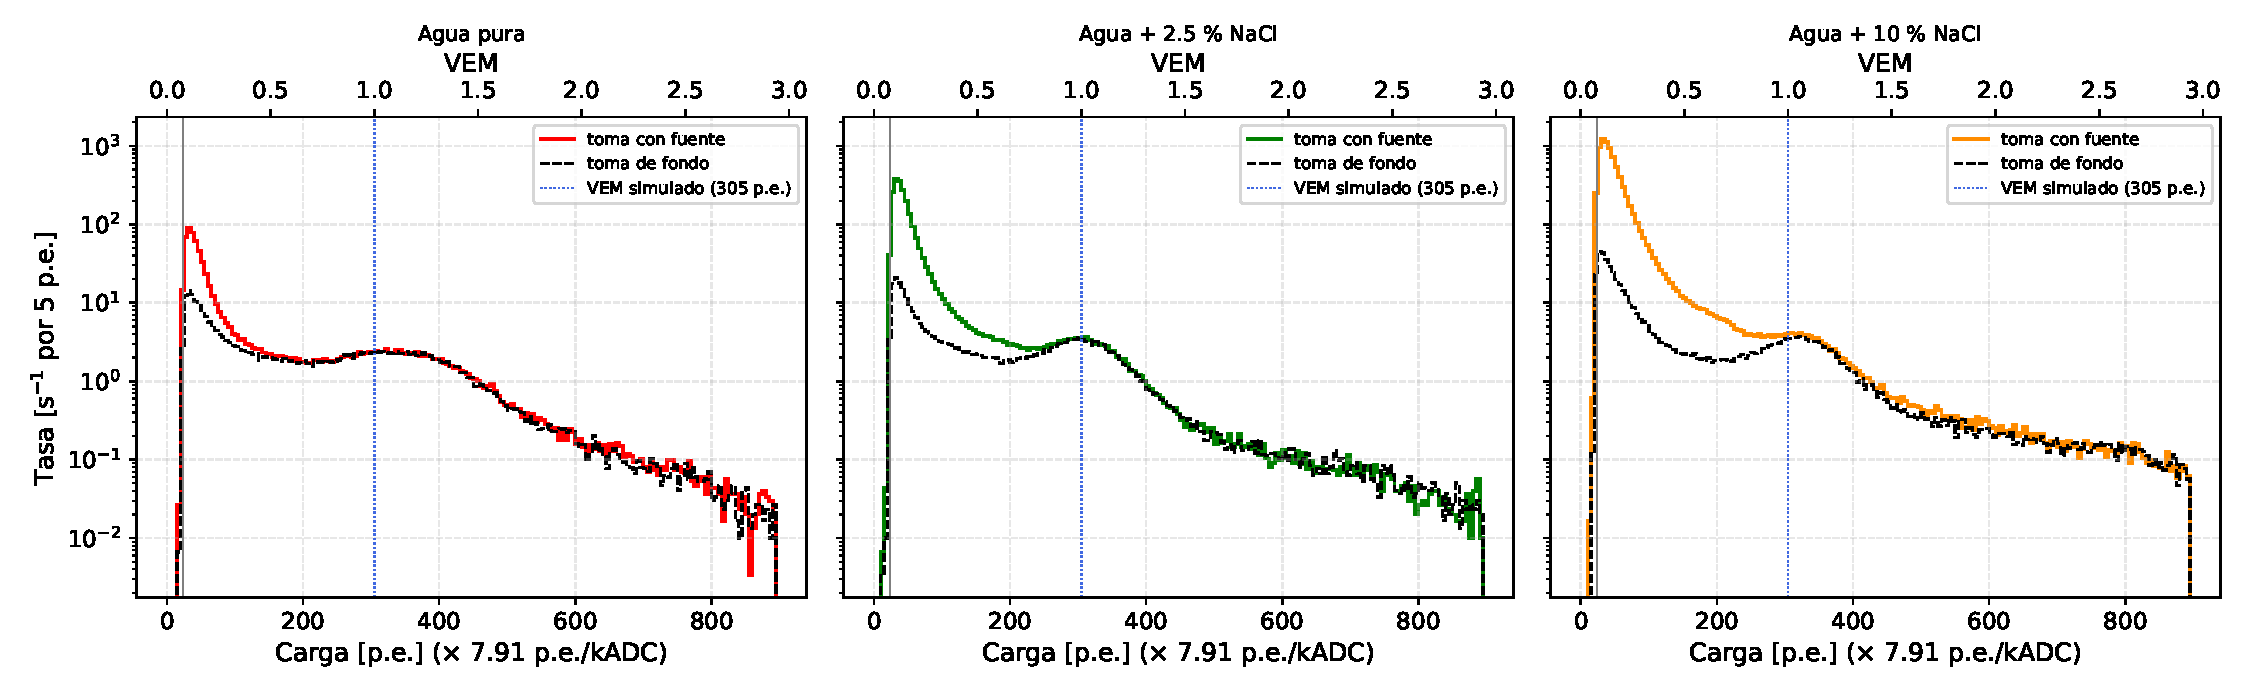
\includegraphics[width=\linewidth]{fig07_bandas_fuente_fondo.pdf}
\caption{Tasa de eventos por carga en la toma con fuente y en la de fondo, con la calibración por muones. Línea
gris: disparo ($\approx$3000~ADC). Línea azul: VEM simulado.}\label{fig:bandas}
\end{figure}

\begin{table}[H]\centering\scriptsize
\tabla{bandas_carga}
\caption{Tasas por banda de carga (método de la ventana del disparo) y cociente fuente/fondo.}\label{tab:bandas}
\end{table}

\subsection{Exceso medido frente a la predicción absoluta}
La figura~\ref{fig:exceso} (izquierda) compara el exceso (toma con fuente menos toma de fondo, en 300~s) con
la predicción absoluta de MEIGA para la fuente de 1~Ci en 5~min. Por debajo del disparo el prototipo no
registra nada, así que solo se puede comparar por encima de $\approx$24~p.e.

\begin{table}[H]\centering\small
\tabla{exceso_vs_meiga}
\caption{Exceso medido entre 23 y 200~p.e.\ (rango entre los dos métodos de carga) y eventos de MEIGA por
encima del disparo para 1~Ci en 300~s. $L$: longitud de caída exponencial del espectro, del exceso medido
(4000--10\,000~ADC) y de la simulación (2--8~p.e.).}\label{tab:exceso}
\end{table}

\begin{figure}[H]\centering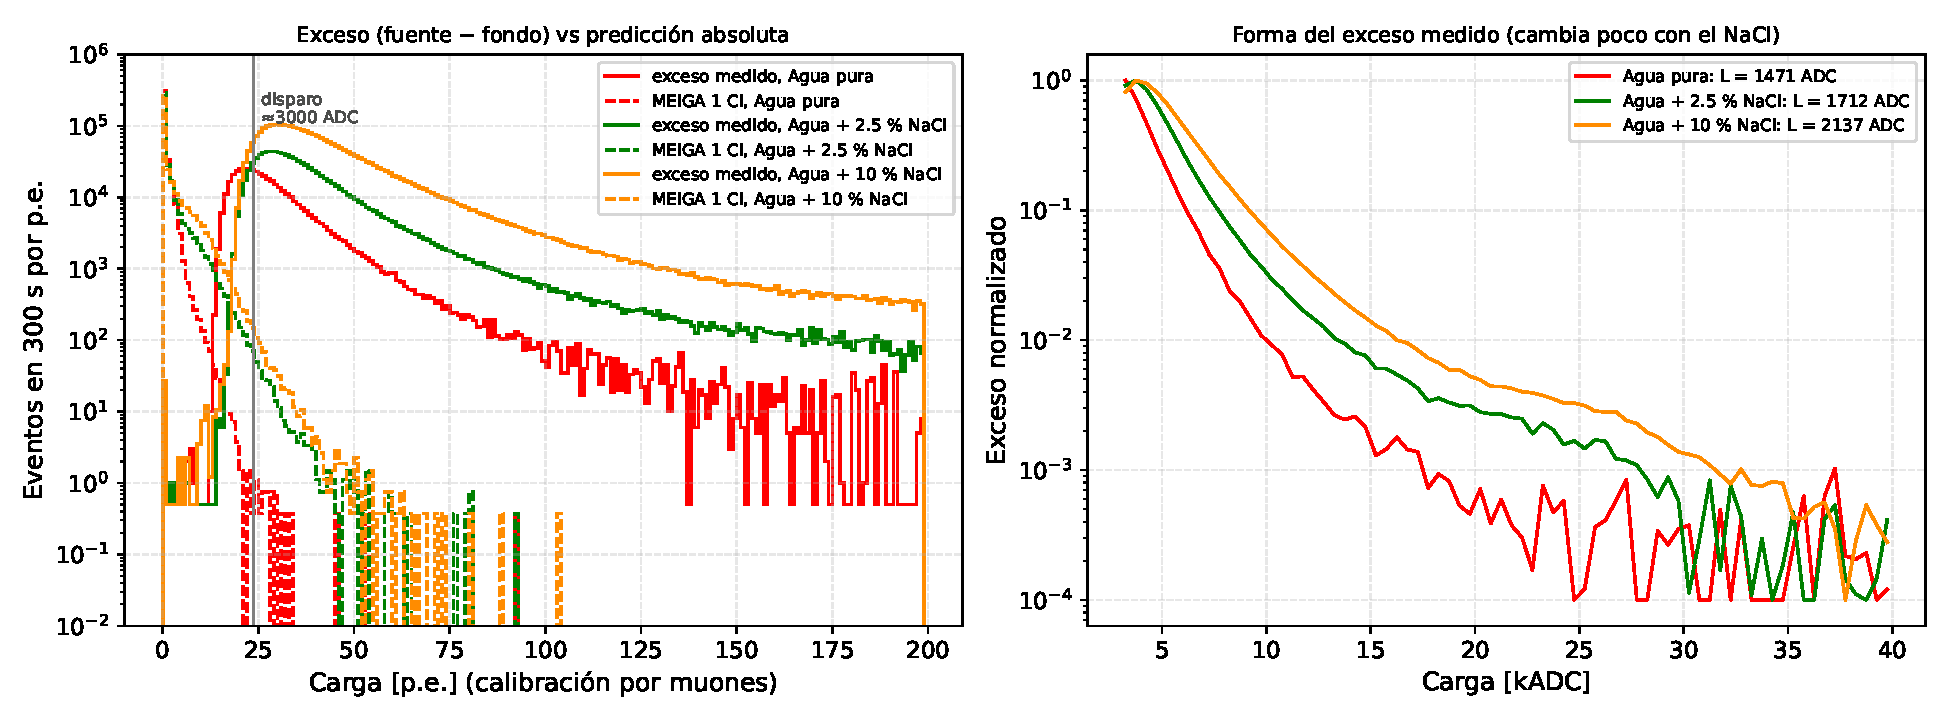
\includegraphics[width=\linewidth]{fig08_exceso_vs_meiga.pdf}
\caption{Izquierda: exceso medido (continuo, método robusto) y predicción absoluta de MEIGA (discontinuo).
Derecha: forma del exceso medido en ADC, normalizada al máximo.}\label{fig:exceso}
\end{figure}

\begin{itemize}
\item Por encima del disparo, el exceso medido es \textbf{$\sim$20\,000--50\,000 veces} lo predicho en
agua pura, \textbf{$\sim$2\,000--4\,000 veces} con 2.5\,\% NaCl y \textbf{$\sim$4\,000--5\,000 veces} con
10\,\% NaCl. Con la calibración antigua (umbral de 12~p.e.) los factores eran 1\,300, 180 y 250
(\archivo{resumen_montaje.json}); la nueva calibración empeora el desacuerdo.
\item La \textbf{forma} tampoco coincide. En la simulación, la longitud de caída del espectro crece un
factor 4.3 de agua pura a 10\,\% NaCl (1.28, 3.07 y 5.53~p.e.). En el experimento crece solo un 30--45\,\%
(de $\approx$1600 a $\approx$1800 y $\approx$2200~ADC). Ajustar la escala para que las formas coincidan
exigiría 0.7--0.9~p.e./kADC en agua pura, 1.6--1.8 con 2.5\,\% y 2.4--2.6 con 10\,\% NaCl: tres calibraciones
distintas, y de 3 a 10 veces menores que la de los muones.
\item Lo que sí sigue la sal es la \textbf{tasa} del exceso: 380--940~s$^{-1}$ (agua pura),
1\,900--3\,100~s$^{-1}$ (2.5\,\%) y 7\,200--9\,400~s$^{-1}$ (10\,\%): cocientes respecto a agua pura de
3--5 y 10--19. En la simulación la señal total ($Q\geq1$) solo sube un 30 y un 70\,\%, pero por encima del
disparo crece mucho más que en el experimento: unas 45 veces (2.5\,\%) y 100 veces (10\,\%).
\end{itemize}

\subsection{Calibración por consistencia entre medios}
Otra forma de calibrar es exigir que el número de neutrones incidentes que implica el experimento,
$N_\text{inc}=\text{detectados}(Q\geq U)/\varepsilon_\text{sim}(Q\geq U)$, sea el mismo en agua pura que en
cada medio con sal (misma fuente, misma geometría). La figura~\ref{fig:consist} barre la calibración de 2 a
14~p.e./kADC para umbrales de 3000 a 6000~ADC.
\begin{itemize}
\item Agua pura frente a 2.5\,\% NaCl: el cociente solo cruza 1 por encima de $\approx$10.7~p.e./kADC y para
umbrales de 5000--6000~ADC, y ahí exige $3\text{--}6\times10^{10}$ neutrones en 5~min.
\item Agua pura frente a 10\,\% NaCl: cruza 1 entre 6.7 y 12.3~p.e./kADC según el umbral, y exige
$1\text{--}6\times10^{10}$ neutrones en 5~min.
\end{itemize}
Son de 15 a 90 veces lo que emite 1~Ci en ese tiempo ($6.7\times10^8$), y los dos pares piden calibraciones
distintas para un mismo umbral (por ejemplo 10.7 y 6.7~p.e./kADC con 6000~ADC). Ninguna calibración hace
coherentes los tres medios con un número de neutrones físico.

\begin{figure}[H]\centering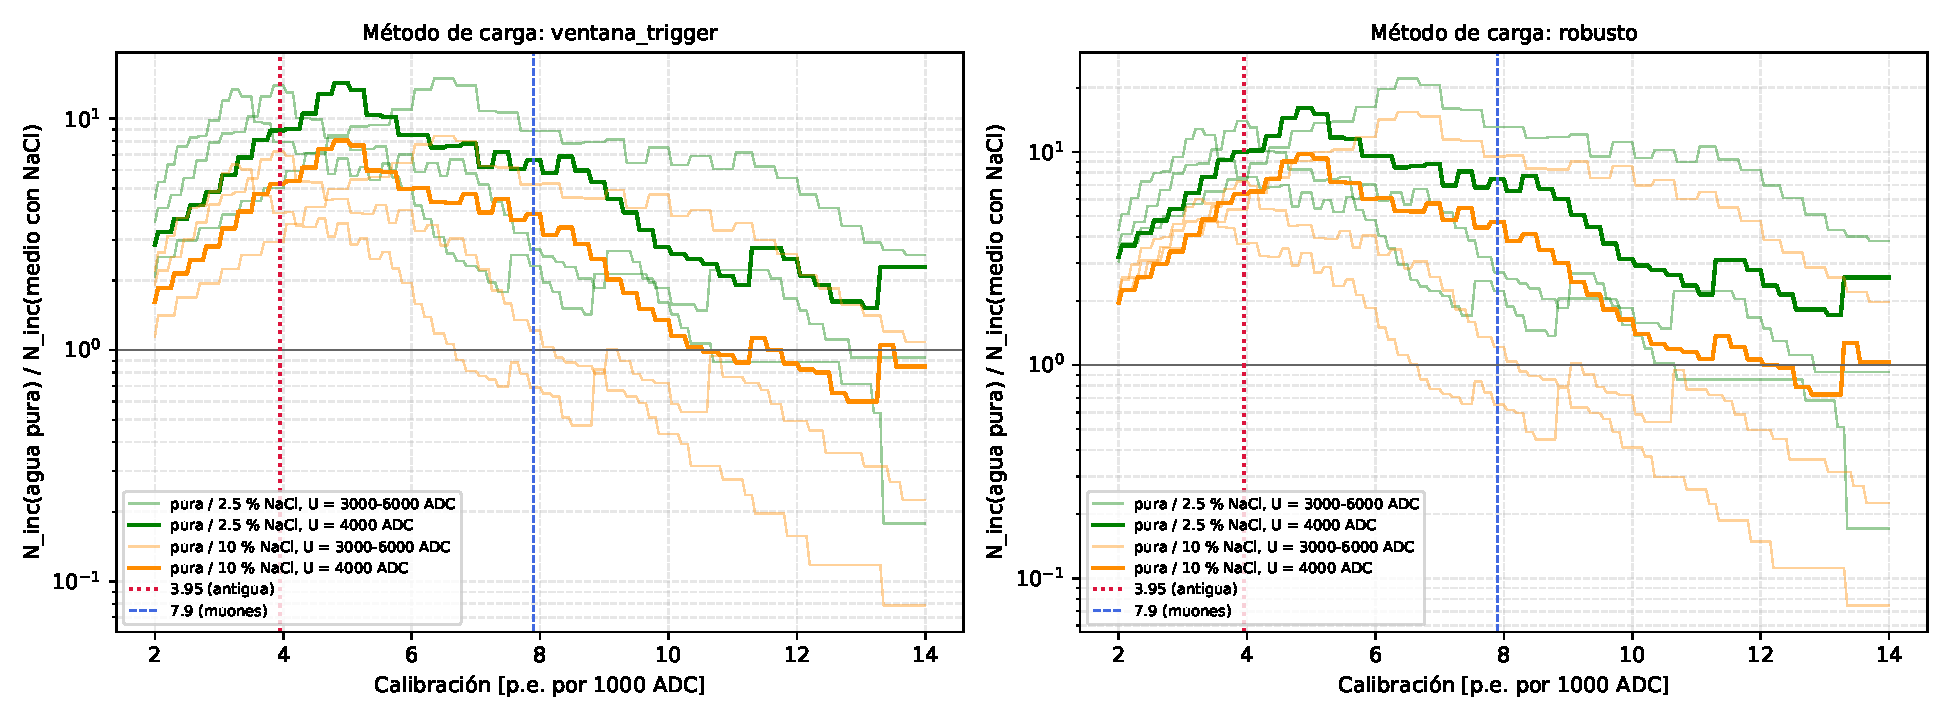
\includegraphics[width=\linewidth]{fig06_calibracion_consistencia.pdf}
\caption{Cociente $N_\text{inc}(\text{pura})/N_\text{inc}(\text{NaCl})$ en función de la calibración, para
2.5\,\% (verde) y 10\,\% NaCl (naranja). Líneas verticales: calibración antigua (3.95) y por muones (7.9).}\label{fig:consist}
\end{figure}

\section{Comparación con el método de los cuadernos del prototipo}\label{sec:cuaderno}
\subsection{El método}
Los cuadernos \archivo{Comparacion-datos-simulado.ipynb} y \archivo{analisis-datos-AmBe-horizontal.ipynb}
(\archivo{Detector-prototipo/Nuevo-analisis/}) comparan los histogramas de carga así:
\begin{enumerate}
\item \textbf{Carga experimental.} Cada disparo se corta en trazas de 32 muestras; se toma la ventana de muestras
positivas que contiene la muestra 8 (el disparo), se conserva el pulso si su pico supera 1200~ADC y la carga es la suma
de la ventana. Es el método ``ventana del disparo'' de este informe: los conteos coinciden exactamente.
\item \textbf{Histograma neto.} Bins de 20~ADC desde 1200~ADC; neto = cuentas de la toma con fuente menos cuentas de
la toma de fondo, sin normalizar por duración.
\item \textbf{Simulación.} Histograma de fotoelectrones por evento, en bins de 1~p.e. El eje horizontal se pasa a ADC
multiplicando por $1000/3.95 = 253$~ADC por p.e. (la calibración antigua de 3.95~p.e./kADC) y el vertical por un factor
de altura (10).
\item \textbf{Principio.} Como explica el grupo, los dos factores son libres, pero deben ser \emph{los mismos para
todos los medios}: el horizontal representa la ganancia del PMT y el vertical el número de neutrones incidentes. Así
no cambia la diferencia relativa entre medios.
\end{enumerate}

\subsection{Reproducción y aplicación al montaje}
La figura~\ref{fig:cuaderno} reproduce el método en tres pasos:
\begin{itemize}
\item \textbf{(a)} El cuaderno con su propia simulación: el archivo \archivo{counts-number-photons.txt}, que no es la
simulación de la fuente Am-Be sino una corrida anterior de \emph{neutrones térmicos} (207\,969 neutrones por medio).
Se reproduce exactamente la figura del cuaderno, con buen acuerdo en los tres medios.
\item \textbf{(b)} Los mismos factores (253~ADC/p.e.\ y $\times10$ por neutrón) con las corridas del montaje Am-Be de
este informe. La simulación queda mucho más estrecha que el experimento: por neutrón, el montaje da la mitad de carga
que la simulación térmica ($\langle Q\rangle$ de 1.95, 3.93 y 5.30~p.e.\ frente a 3.69, 7.71 y 10.58~p.e.), porque los
neutrones entran por el costado y se capturan lejos del PMT de la tapa.
\item \textbf{(c)} El montaje con factores comunes \emph{ajustados} a los tres medios a la vez (exceso neto entre 4500 y
30\,000~ADC, escala logarítmica, resolución de 1~p.e.\ del 40\,\%; los bins sin eventos simulados cuentan como medio
evento; \archivo{scripts/ajuste_factor_comun.py}):
\textbf{975--1050~ADC/p.e.\ y $4.7$--$6.6\times10^6$ neutrones incidentes en 300~s}, según el método de carga. El
agua pura coincide en forma e intensidad sin ningún desplazamiento; con 2.5\,\% NaCl la simulación queda unas 2 veces
por encima entre 8\,000 y 20\,000~ADC, y con 10\,\% cae más rápido que el experimento por encima de 25\,000~ADC
(figura~\ref{fig:comun}). Si se deja libre solo el factor vertical de cada medio, salen 7.5, 2.7 y
$5.7\times10^6$ neutrones (pura, 2.5 y 10\,\%; método de la ventana del disparo).
\end{itemize}

\begin{figure}[H]\centering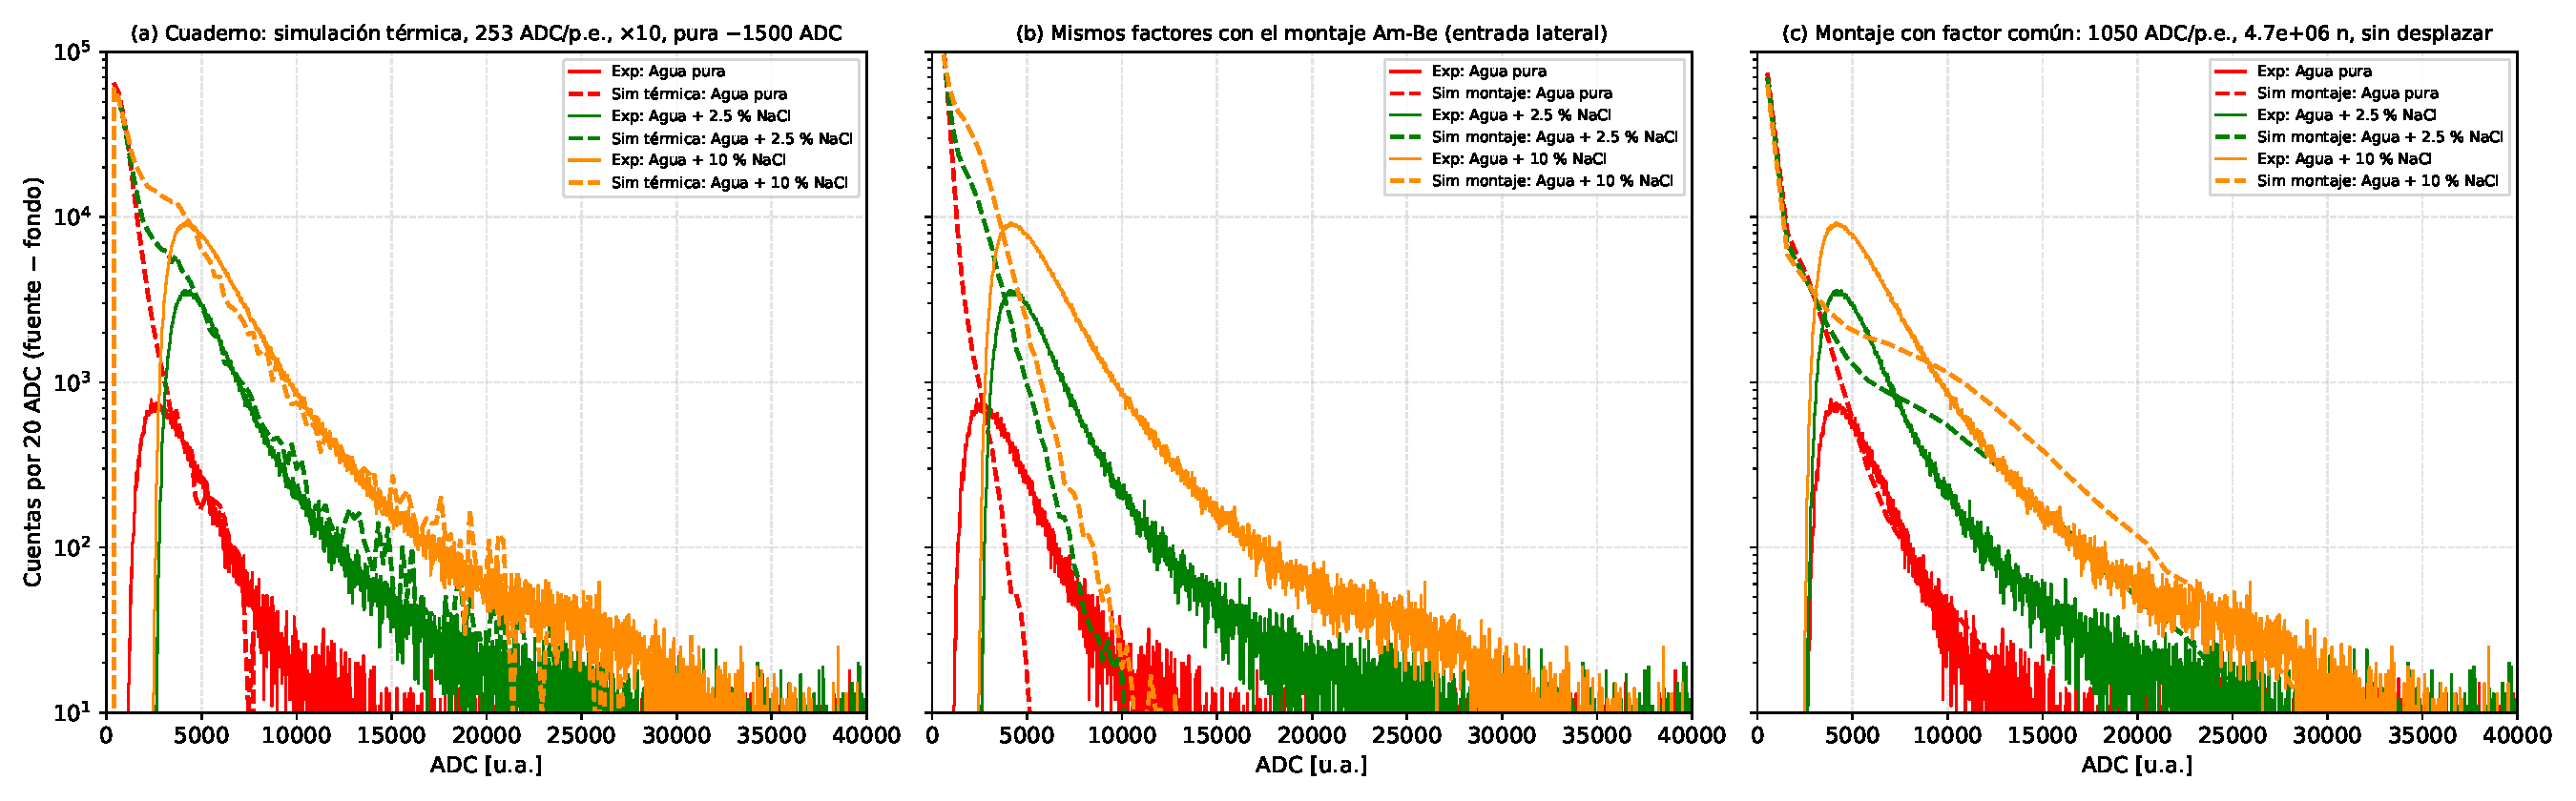
\includegraphics[width=\linewidth]{fig11_metodo_cuaderno.pdf}
\caption{Método de los cuadernos. (a) Simulación térmica del cuaderno, 253~ADC/p.e., $\times10$, agua pura desplazada
$-1500$~ADC. (b) Mismos factores con el montaje Am-Be. (c) Montaje con el factor común ajustado, sin desplazar el
agua pura. Continuo: experimento (fuente $-$ fondo); discontinuo: simulación.}\label{fig:cuaderno}
\end{figure}

\begin{figure}[H]\centering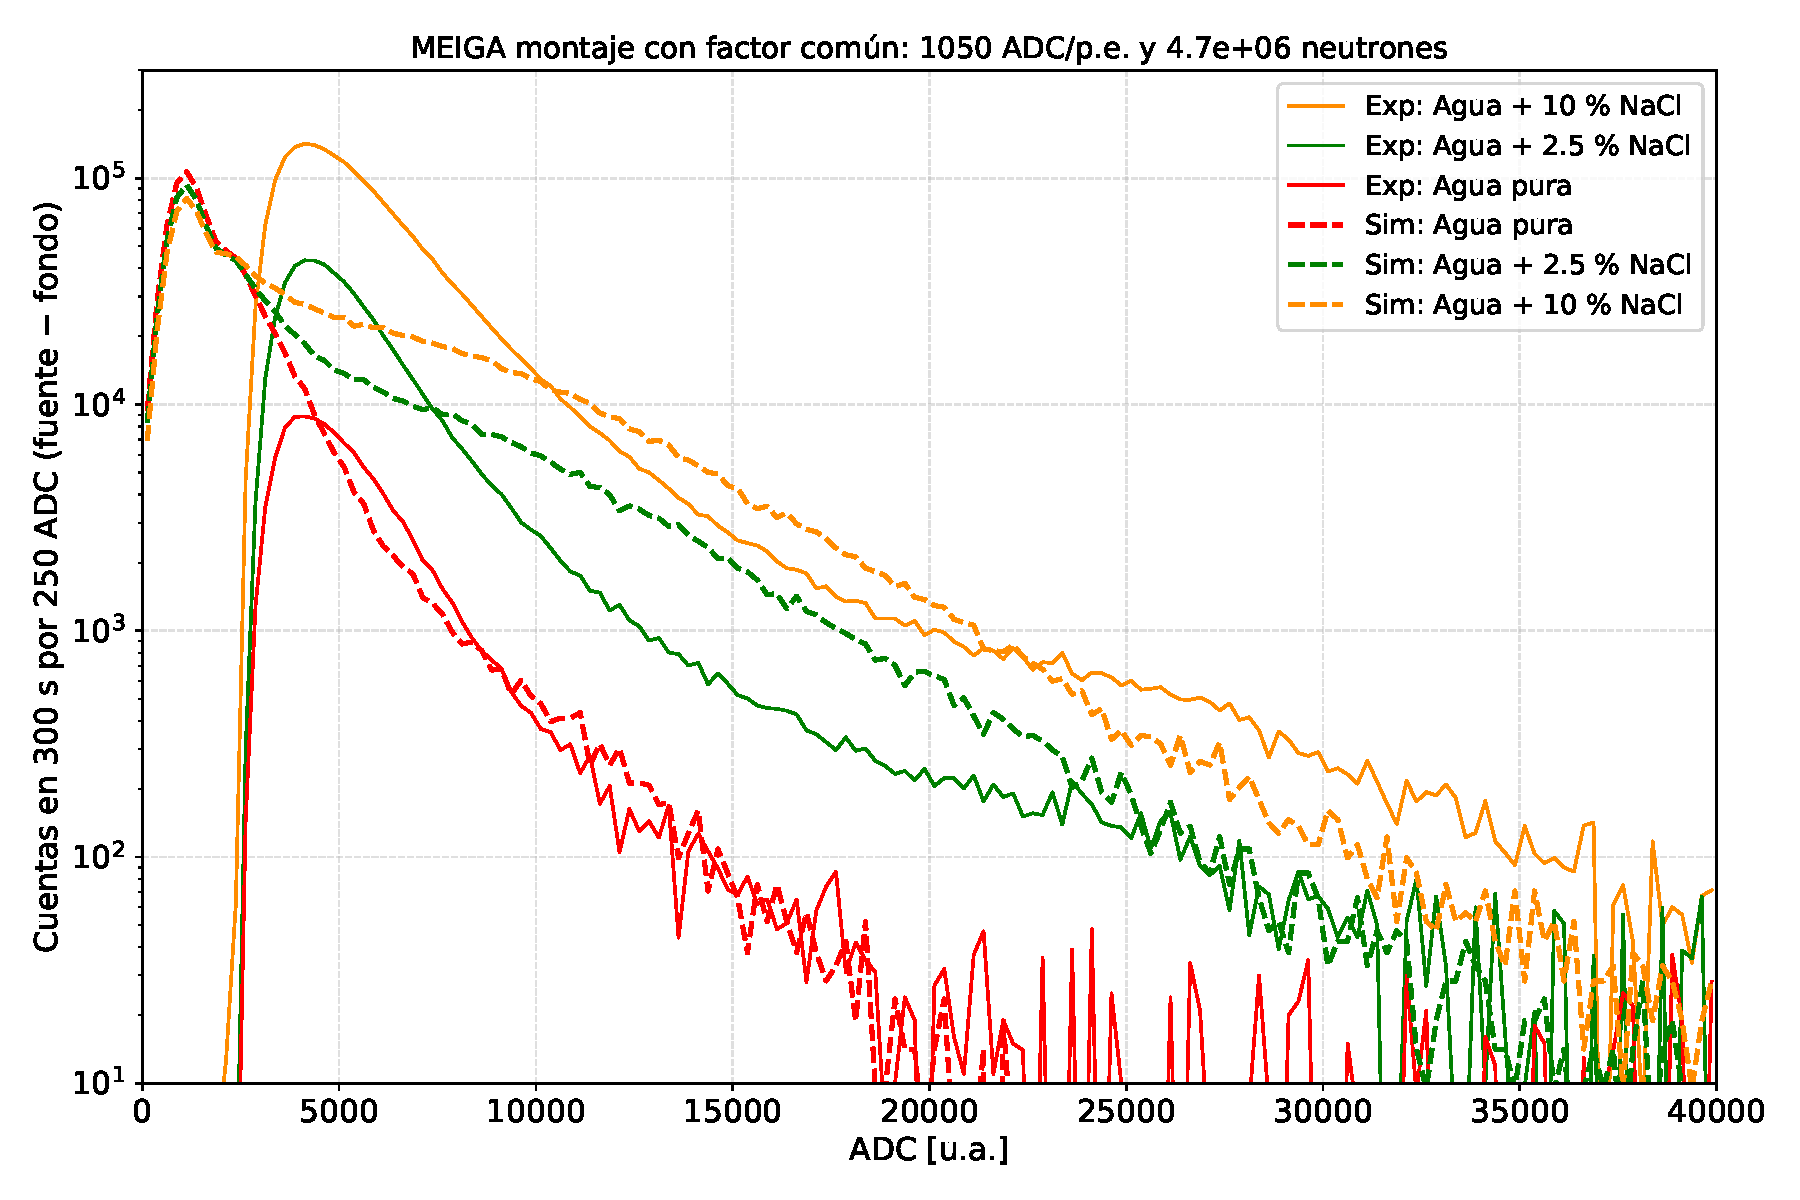
\includegraphics[width=0.85\linewidth]{fig10b_histogramas_factor_comun.pdf}
\caption{Histogramas de carga del montaje con el factor común (1050~ADC/p.e., $4.7\times10^6$ neutrones en 300~s; exceso
normalizado a 300~s, bins de 250~ADC).}\label{fig:comun}
\end{figure}

\subsection{Corridas de la Campaña~1 (inyección por la tapa)}\label{sec:c1}
El mismo ajuste se aplicó a las 16 corridas monoenergéticas de la Campaña~1: 100\,000 neutrones por corrida y medio,
inyectados verticalmente por la tapa, de 1~meV a 1~keV (\archivo{Carga/<E>/Carga_Total_*.txt};
\archivo{scripts/ajuste_factor_comun_campana1.py}). Como la ganancia del PMT es una sola, el factor horizontal se
ajustó común a todas las energías y el vertical libre para cada una (figuras~\ref{fig:c1} y~\ref{fig:c1f}):
\begin{itemize}
\item \textbf{Factor horizontal global: 450~ADC/p.e.} (2.2~p.e./kADC). Ajustado energía por energía sale entre 400 y
575, sin tendencia con la energía.
\item \textbf{Neutrones incidentes: $5.5$--$10\times10^6$ en 300~s}, algo más para las energías más bajas (1--10~meV).
\item La forma simulada casi no depende de la energía del neutrón ($\langle Q\rangle$ de 3.2, 7.5 y 10.5~p.e.\ en
pura, 2.5 y 10\,\% en todas las energías), de modo que todas las energías dan el mismo acuerdo: rms de
$\ln(\text{exp}/\text{sim})$ entre 0.70 y 0.77, un factor $\approx2$.
\item \textbf{10\,\% NaCl} coincide muy bien en forma e intensidad por encima de 8\,000~ADC; con \textbf{2.5\,\%} la
simulación queda unas 2 veces por encima; en \textbf{agua pura} la simulación cae unas 3 veces más rápido que el
experimento, igual que con el montaje: el agua pura medida tiene una cola más larga que la que da la simulación.
\end{itemize}
El factor horizontal con las corridas por la tapa (450~ADC/p.e.) es menor que con el montaje (1000) porque, con el PMT
y la geometría de la Campaña~1, cada neutrón con señal deja de 1.6 a 2 veces más carga. Sigue siendo 3.6 veces el valor de los muones.

\begin{figure}[H]\centering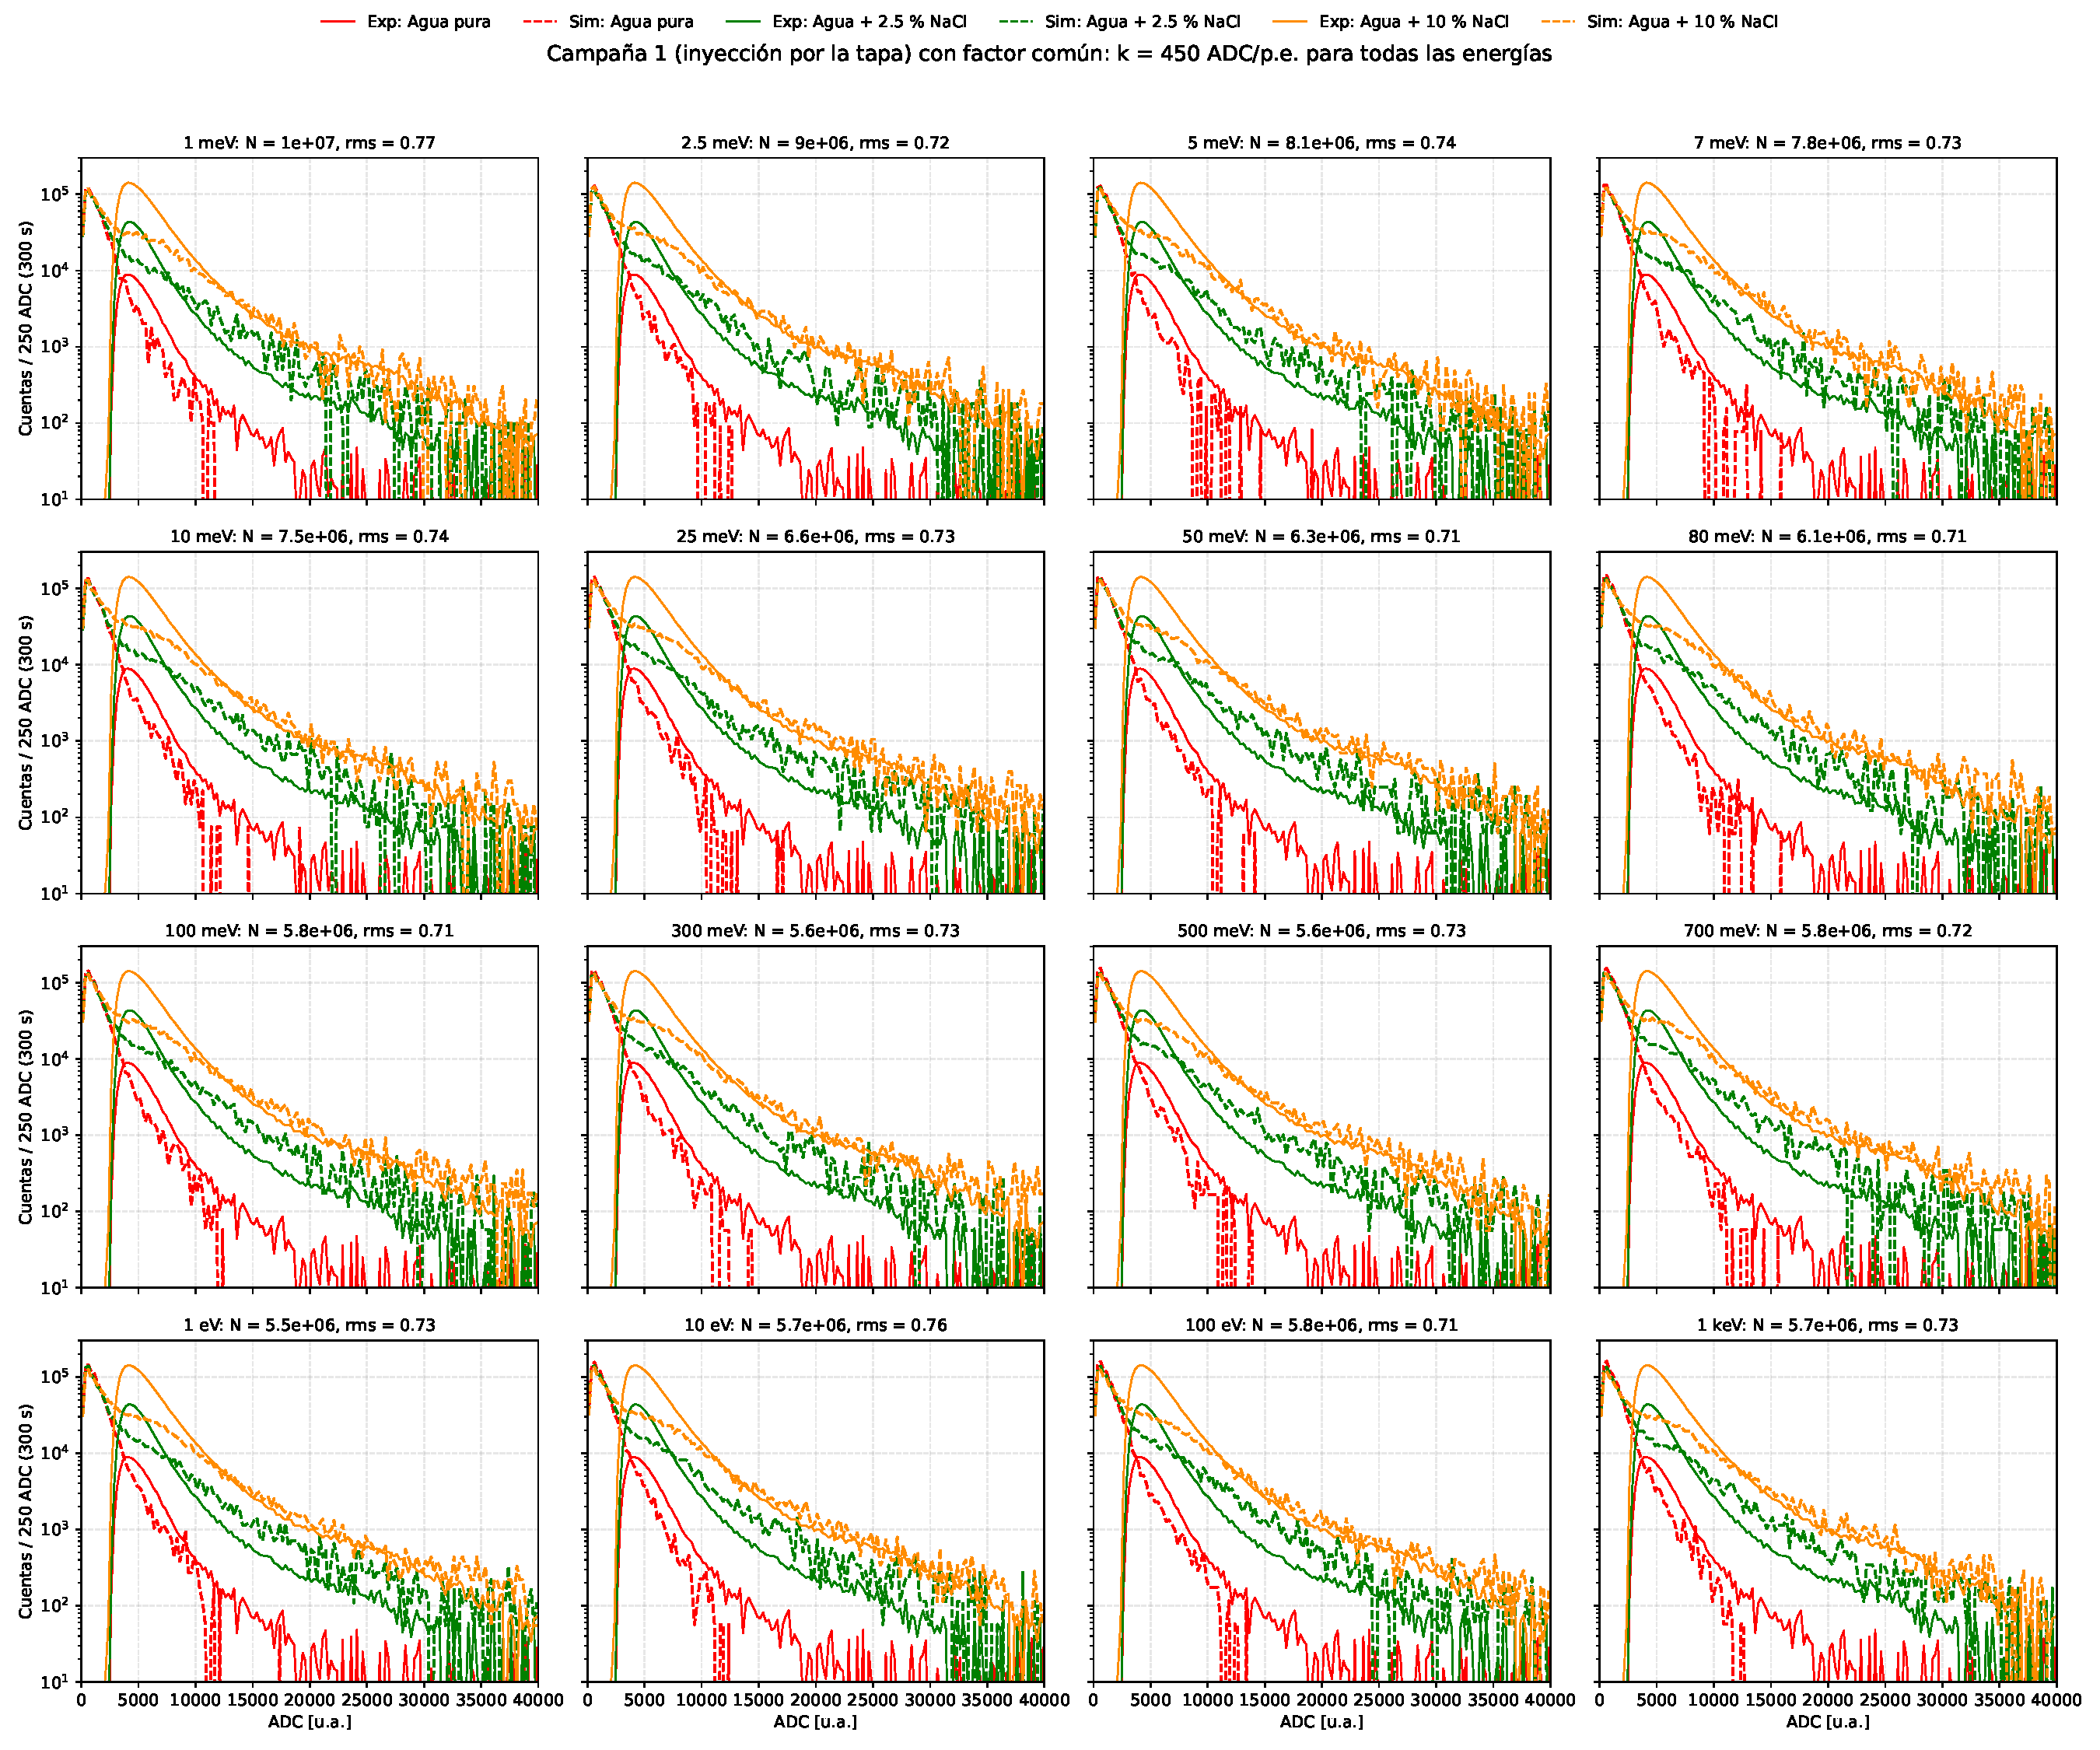
\includegraphics[width=\linewidth]{fig12_campana1_factor_comun.pdf}
\caption{Corridas de la Campaña~1 (inyección por la tapa, 1~meV--1~keV) con un factor horizontal común (450~ADC/p.e.)
y el número de neutrones de cada energía. Continuo: experimento (fuente $-$ fondo, 300~s); discontinuo: simulación.}\label{fig:c1}
\end{figure}
\begin{figure}[H]\centering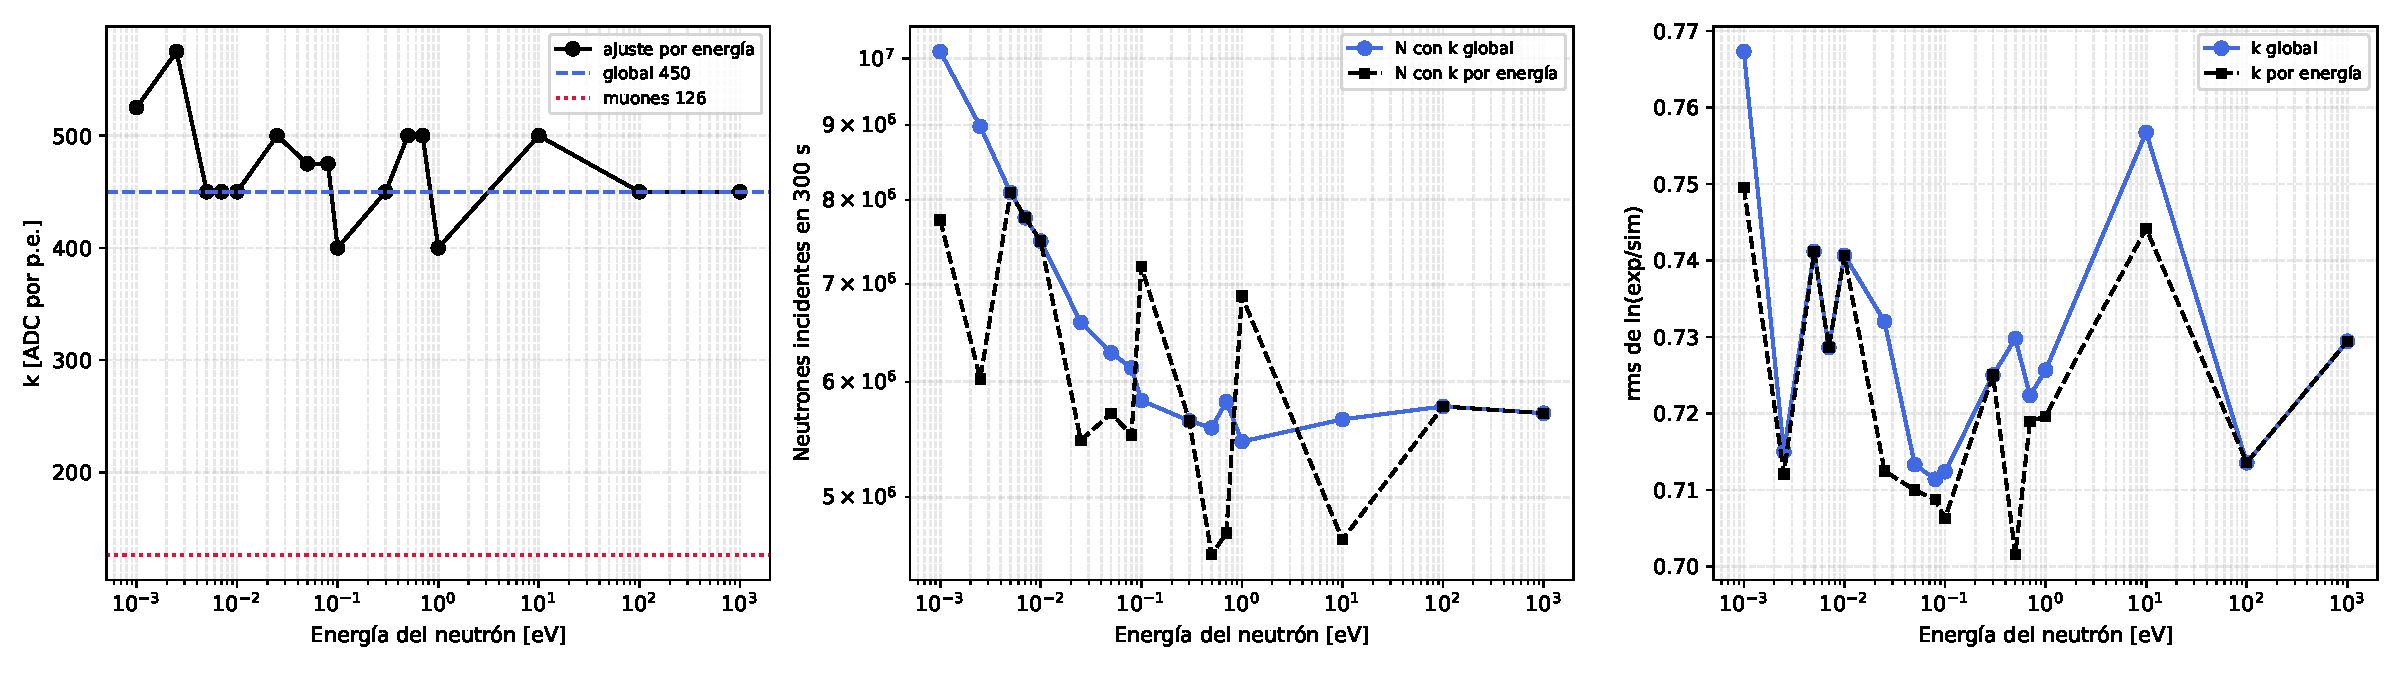
\includegraphics[width=\linewidth]{fig13_campana1_factores.pdf}
\caption{Campaña~1: factor horizontal, neutrones incidentes y calidad del ajuste frente a la energía del neutrón.}\label{fig:c1f}
\end{figure}

\subsection{Observaciones}
\begin{enumerate}
\item \textbf{Desplazamiento del agua pura.} Los dos cuadernos desplazan el agua pura experimental $-1500$~ADC
(\texttt{SHIFT\_ADC\_PURA}). Eso contradice el principio de un mismo factor para todos los medios. Con el montaje y el
factor común ajustado no hace falta desplazarla.
\item \textbf{Columna de 10\,\%.} En \archivo{analisis-datos-AmBe-horizontal.ipynb} el archivo simulado tiene cinco
columnas (pura, 2.5, 5 y 10\,\%) y se leen las cuatro primeras (\texttt{usecols=[0,1,2,3]}): la curva rotulada
``10\,\%'' es en realidad la de 5\,\%. \archivo{Comparacion-datos-simulado.ipynb} lee bien las columnas.
\item \textbf{Duración.} La toma con fuente de 10\,\% dura 240~s y su fondo 299~s; restar conteos sin normalizar
cambia el neto en un 1.6\,\%, poco frente a las diferencias discutidas.
\item \textbf{Factores distintos según la simulación.} El factor horizontal que hace coincidir las formas depende de la
simulación usada: 253~ADC/p.e.\ en el cuaderno con la simulación térmica, 450 al ajustarlo a las corridas de la
Campaña~1 (sección~\ref{sec:c1}) y unos 1000 con el montaje Am-Be. El factor común, por sí solo,
no fija la ganancia real del PMT.
\item \textbf{Tensión con los muones.} Con 1000~ADC/p.e.\ un muón vertical simulado (305~p.e.) daría unos 300~kADC,
pero el pico de muones medido está en unos 40~kADC (127--140~ADC/p.e.). La comparación con factor común es coherente
entre medios, pero no a la vez con los muones: la luz por MeV de las capturas en el experimento es unas 8 veces mayor,
relativa a los muones, que en la simulación.
\item \textbf{Neutrones incidentes.} Los $4.7$--$6.6\times10^6$ neutrones en 300~s del ajuste son de 13 a 18 veces los
del modelo de blindaje para 1~Ci (373\,272) y un 0.7--1.0\,\% de lo que emite la fuente.
\end{enumerate}

\section{Interpretación}
En la escala de los muones, el exceso medido se extiende de 0.08 a 0.7~VEM, es decir, de $\approx$20 a
$\approx$200~MeV de electrón equivalente. La fuente no tiene nada que deposite tanta energía en forma de luz
Cherenkov:
\begin{itemize}
\item el gamma de captura en H es de 2.2~MeV y la cascada del $^{36}$Cl suma 8.6~MeV, repartida en varios
gammas;
\item el gamma de 4.44~MeV del $^{12}$C$^*$ de la reacción $^9$Be$(\alpha,n)$ (unos 0.6 por neutrón), que
estas simulaciones no incluyen, daría típicamente $\approx$5~p.e.\ ($\approx$0.015~VEM): \textbf{no basta}
para explicar el exceso, aunque aporte por debajo del disparo;
\item los protones de retroceso de los neutrones rápidos (hasta 11~MeV) están por debajo del umbral
Cherenkov.
\end{itemize}

Como la región de muones se resta perfectamente, la ganancia y la normalización de las tomas no explican la
discrepancia. Quedan tres hipótesis, que se pueden comprobar con los datos crudos o con medidas sencillas:
\begin{enumerate}
\item \textbf{No linealidad o saturación del PMT o de la electrónica} para los pulsos grandes. Si el pico de
muones estuviera comprimido, la calibración con muones sobrestimaría los p.e.\ de los pulsos pequeños. La
calibración por forma (0.7--1.8~p.e./kADC) indicaría una compresión de 5--10 veces. Se comprueba con el
pico de un fotoelectrón (LED o pulsos sin disparo), o con la carga de muones frente a la amplitud de pico.
\item \textbf{Apilamiento de pulsos} dentro de la ventana de integración: con fuente, la tasa de disparo sube
de $\approx$400 a 1\,900 (pura), 3\,700 (2.5\,\%) y 10\,400~s$^{-1}$ (10\,\%). Eso concuerda con que el exceso
crezca más que la señal simulada. Se comprueba con la distribución de tiempos entre disparos y con el número de
pulsos por traza.
\item \textbf{Interacción directa en el PMT o en su base} (gammas y neutrones de la fuente que llegan al
vidrio o al fotocátodo): la simulación solo cuenta fotones ópticos producidos en el agua.
\end{enumerate}

\aviso{En el informe anterior se planteó que el gamma de 4.44~MeV podía explicar la señal alta en agua pura.
Con la escala de los muones esa hipótesis no alcanza (típicamente 5~p.e.\ frente a 24--200~p.e.). Se mantiene como
contribución por debajo del disparo y como ingrediente que falta en la simulación de la fuente.}

\section{Conclusiones}
\begin{enumerate}
\item La entrada lateral da menos señal que la entrada por la tapa: $\varepsilon(Q\geq1)$ total de 17.5\,\% (agua
pura), 22.7\,\% (2.5\,\% NaCl) y 29.8\,\% (10\,\% NaCl), con cargas medias de 1.95, 3.93 y 5.30~p.e.; con
10\,\% NaCl el $^{35}$Cl recibe el 67.5\,\% de las capturas.
\item La calibración por muones da 7.9~p.e./kADC (7.5--8.6), el doble de la usada hasta ahora; el disparo
del prototipo queda en $\approx$24~p.e.
\item Las tomas del prototipo son coherentes entre sí (los muones se restan a cero), pero el exceso con fuente
está entre 0.08 y 0.7~VEM, donde la simulación no predice casi nada. Ni la calibración por muones ni la de
consistencia entre medios lo resuelven: la diferencia está en el detector real o en la lectura, no en la escala.
\item Con el método de los cuadernos (factores comunes) el montaje reproduce los tres medios dentro de un factor 2,
con $\approx$1000~ADC/p.e.\ y $5$--$7\times10^6$ neutrones en 300~s, sin desplazar el agua pura. El acuerdo de la figura de los
cuadernos se obtuvo con una simulación de neutrones térmicos, no con la del montaje Am-Be. El factor horizontal
ajustado es unas 8 veces el de los muones (450~ADC/p.e., 3.6 veces, con las corridas de la Campaña~1 por la tapa):
esa tensión es la pregunta abierta.
\item Siguiente paso experimental: medir el pico de un fotoelectrón y la linealidad, y revisar el apilamiento
en las trazas crudas de las tomas con fuente.
\item La corrida de 10\,\% NaCl confirma el diagnóstico: en la simulación la sal alarga mucho la cola de carga,
y en el experimento casi no la cambia; lo que sí crece con la sal es la tasa del exceso.
\end{enumerate}

\section*{Archivos}
\begin{itemize}
\item \archivo{scripts/procesar_montaje.py}: corrida (4 partes) $\to$ \archivo{resultados/eventos_<medio>.npz}.
\item \archivo{scripts/analizar_montaje.py}: respuesta por componente, modelo de 5~min, figura~\ref{fig:carga}.
\item \archivo{scripts/calibrar_vem.py}: calibración con muones (\archivo{calibracion_vem.json}, figura~\ref{fig:vem}).
\item \archivo{scripts/calibracion_por_consistencia.py}: figura~\ref{fig:consist}.
\item \archivo{scripts/comparar_con_calibracion_vem.py}: bandas, exceso frente a MEIGA (figuras~\ref{fig:bandas} y~\ref{fig:exceso}).
\item \archivo{scripts/ajuste_factor_comun.py}: ajuste de factores comunes (figura~\ref{fig:comun}).
\item \archivo{scripts/ajuste_factor_comun_campana1.py}: factores comunes con las corridas de la Campaña~1 (figuras~\ref{fig:c1} y~\ref{fig:c1f}).
\item \archivo{scripts/comparacion_metodo_cuaderno.py}: reproducción del método de los cuadernos (figura~\ref{fig:cuaderno}).
\item \archivo{scripts/tablas_informe.py}: tablas de este informe a partir de los JSON.
\item \archivo{Analisis-montaje-MEIGA.ipynb}: cuaderno que ejecuta todo y muestra los resultados.
\end{itemize}
\end{document}
